\documentclass[]{article}
\usepackage{graphicx}
\usepackage{hyperref}
%opening
\title{Stress Testing Ed-HMI220-070C}
\author{Nyle Controls Group}

\begin{document}

\maketitle

\begin{abstract}
In an effort to better detect behaviours of products at the limits of our operational range, we are stress testing devices at max loads for extended periods of time.
\textbf{TLDR: HMI Max temp:87.1 °C (188.78 °F) while in a sealed and insulated box}
The screen may behave like a heat sink, and orientation may impact cooling. at 100\% lodad
the HMI trends towards 61°C (140 °F) 

\end{abstract}

\section*{Method}
The Ed-HMI220-070C in this testing sequence was subjugated to 100\% CPU load for the duration of the workday 3.23.26 packed in an insulated box with 0 ventilation. \\
At the end of the day the Ed-HMI220-070C was removed from that box, and left running at 100\% CPU load overnight.

\section*{Tools}

     \begin{verbatim}
	$ sudo apt install stress-ng lm-sensors
\end{verbatim}
also get: \\ \url{https://github.com/elovejoy-nyle/loadTest/blob/main/cpu_burn.sh}\\
which is a modified script from the authors of stress-ng package, with inclusions of logging.\\ 

lm-sensors was pre-configured on the distro which shipped with this device, if it were not, you would run:
\begin{verbatim}
 sudo sensors-detect --auto
\end{verbatim}
\section*{Results}

Nominal Run Time: 3 Days, in factory intended orientation, peak Temperature: 110F under not load
HMI Max temp:87.1 °C (188.78 °F) while in an insulated, unventilated box. 
	 	\begin{figure}[h!]
	\centering
	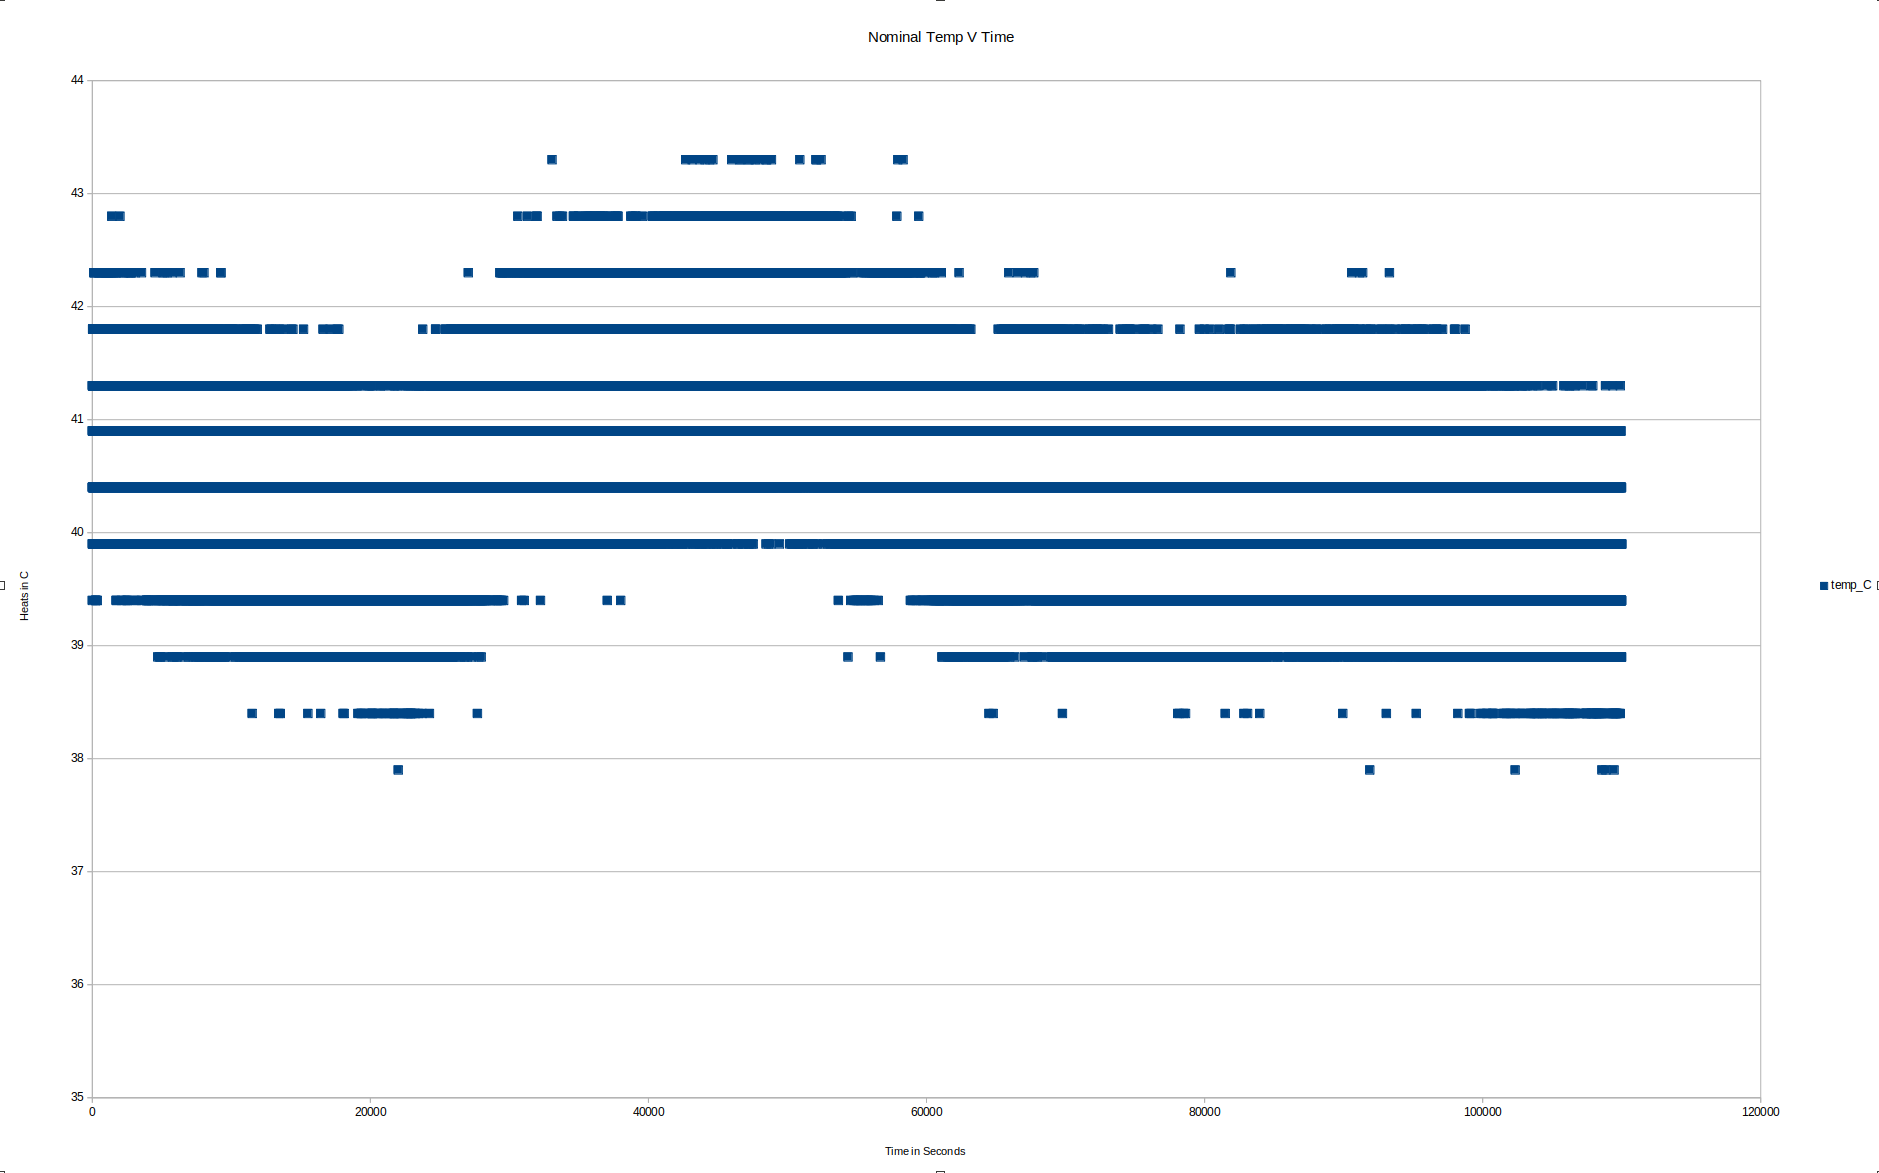
\includegraphics[width=1.0\linewidth]{noLoad.png}
	\caption{1.25 Day, no load thermals}
	%\label{fig:1}
\end{figure}


	 	\begin{figure}[h!]
	\centering
	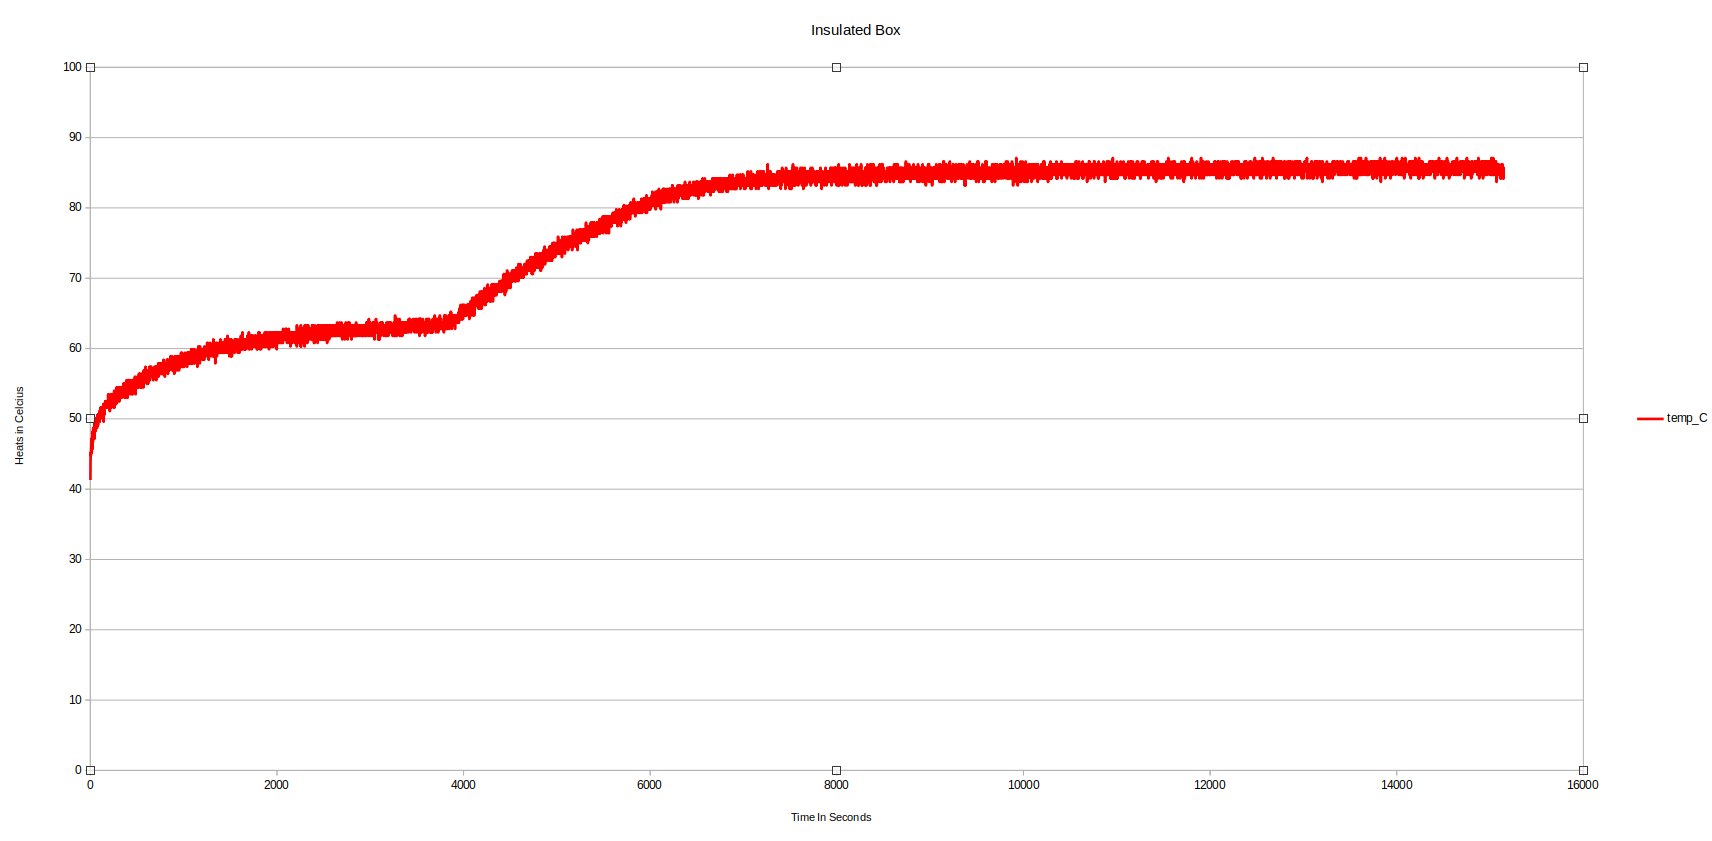
\includegraphics[width=1.0\linewidth]{insulated.png}
	\caption{HMI in insulated box. Bump is where lid was closed}
	%\label{fig:1}
\end{figure}




\begin{figure}[h!]
	\centering
	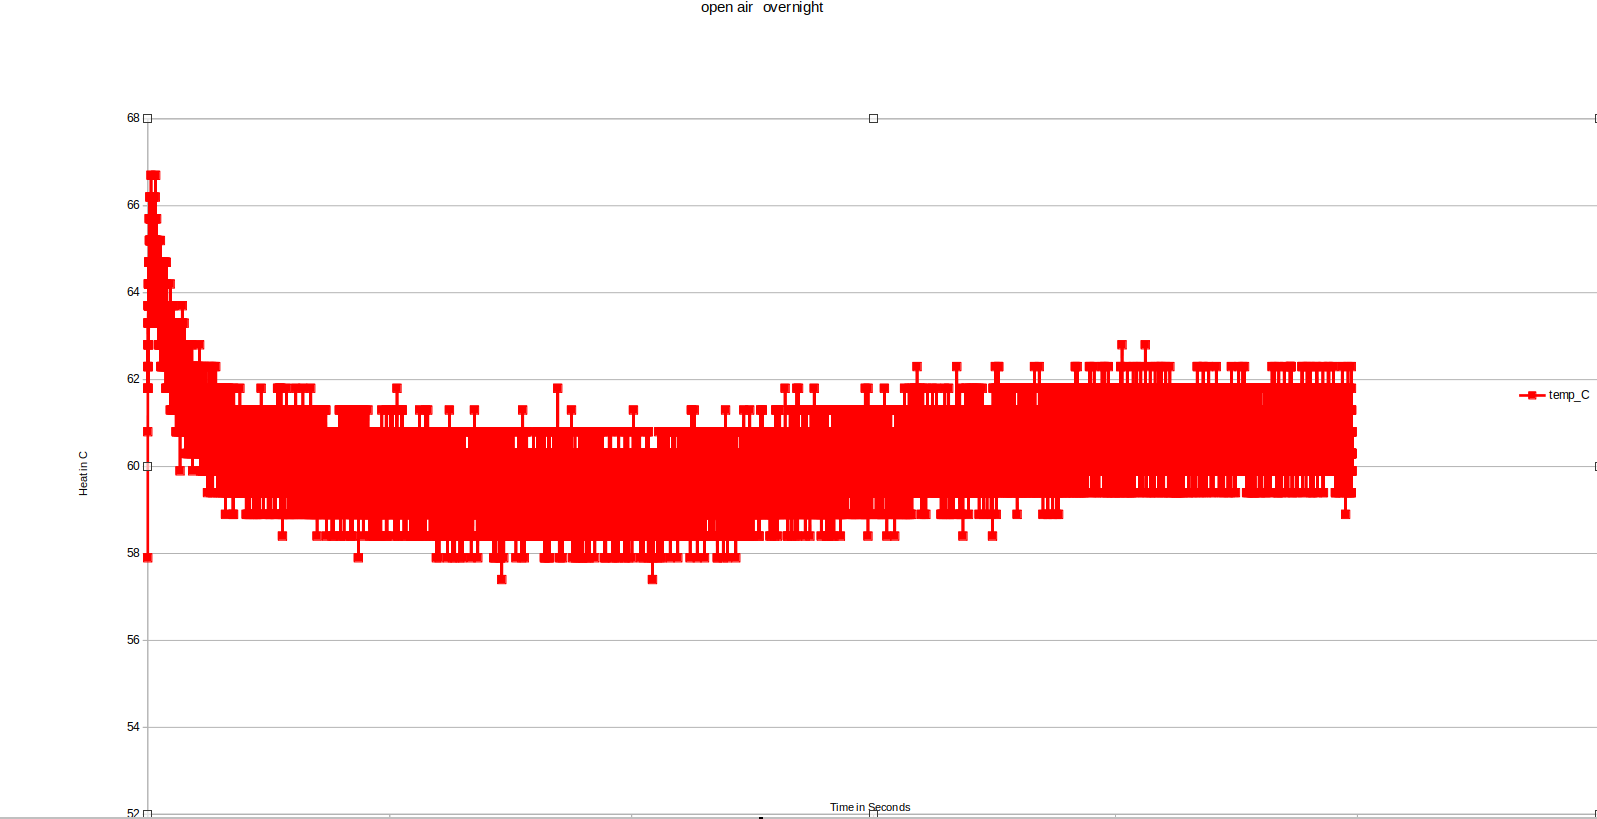
\includegraphics[width=1.0\linewidth]{overNight.png}
	\caption{Test began immediately after insulated box testing}
	%\label{fig:1}
\end{figure}

\begin{figure}[h!]
	\centering
	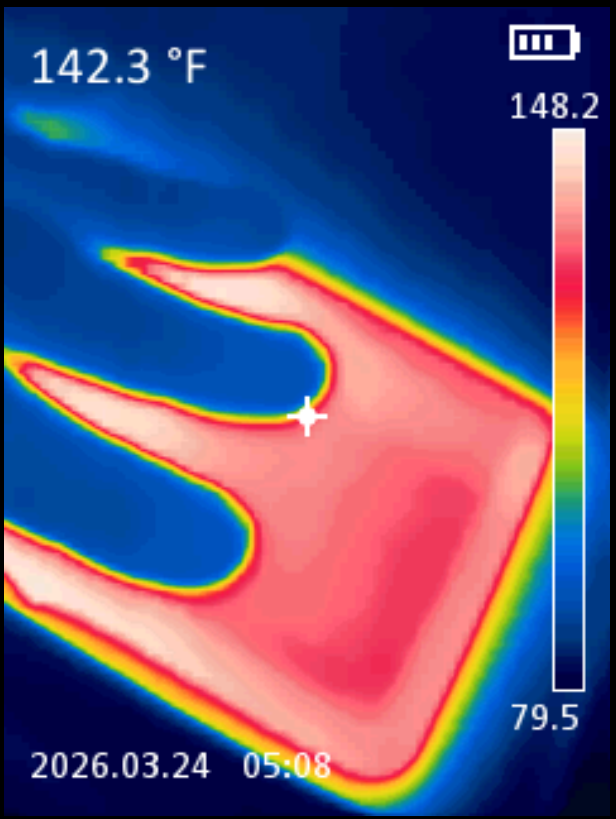
\includegraphics[width=1.0\linewidth]{coolhandluke.png}
	\caption{Human hand for contrast, after insulated test}
	%\label{fig:1}
\end{figure}



\end{document}
